%==============================================================
%  Figura 8.9 - Combinazione di un equipaggiamento di comando
%  elettromeccanico e di un semplice dispositivo di frenatura
%  elettronico per l'arresto di macchine per la lavorazione del
%  legno (Esempio 4)
%  Adattamento in italiano della Figura 8.9 dell'IFA Report 2/2017
%
%  I simboli riproducono quelli dell'originale: le coordinate sono
%  ricavate dal disegno di partenza (1 cm = 70 px, origine
%  nell'angolo in alto a sinistra della cornice). Nessun cambio di
%  corpo del font: le etichette sono ingrandite con "scale" (vedere
%  la nota nella Figura 8.3).
%==============================================================
\definecolor{verdemotore}{RGB}{22,67,38}
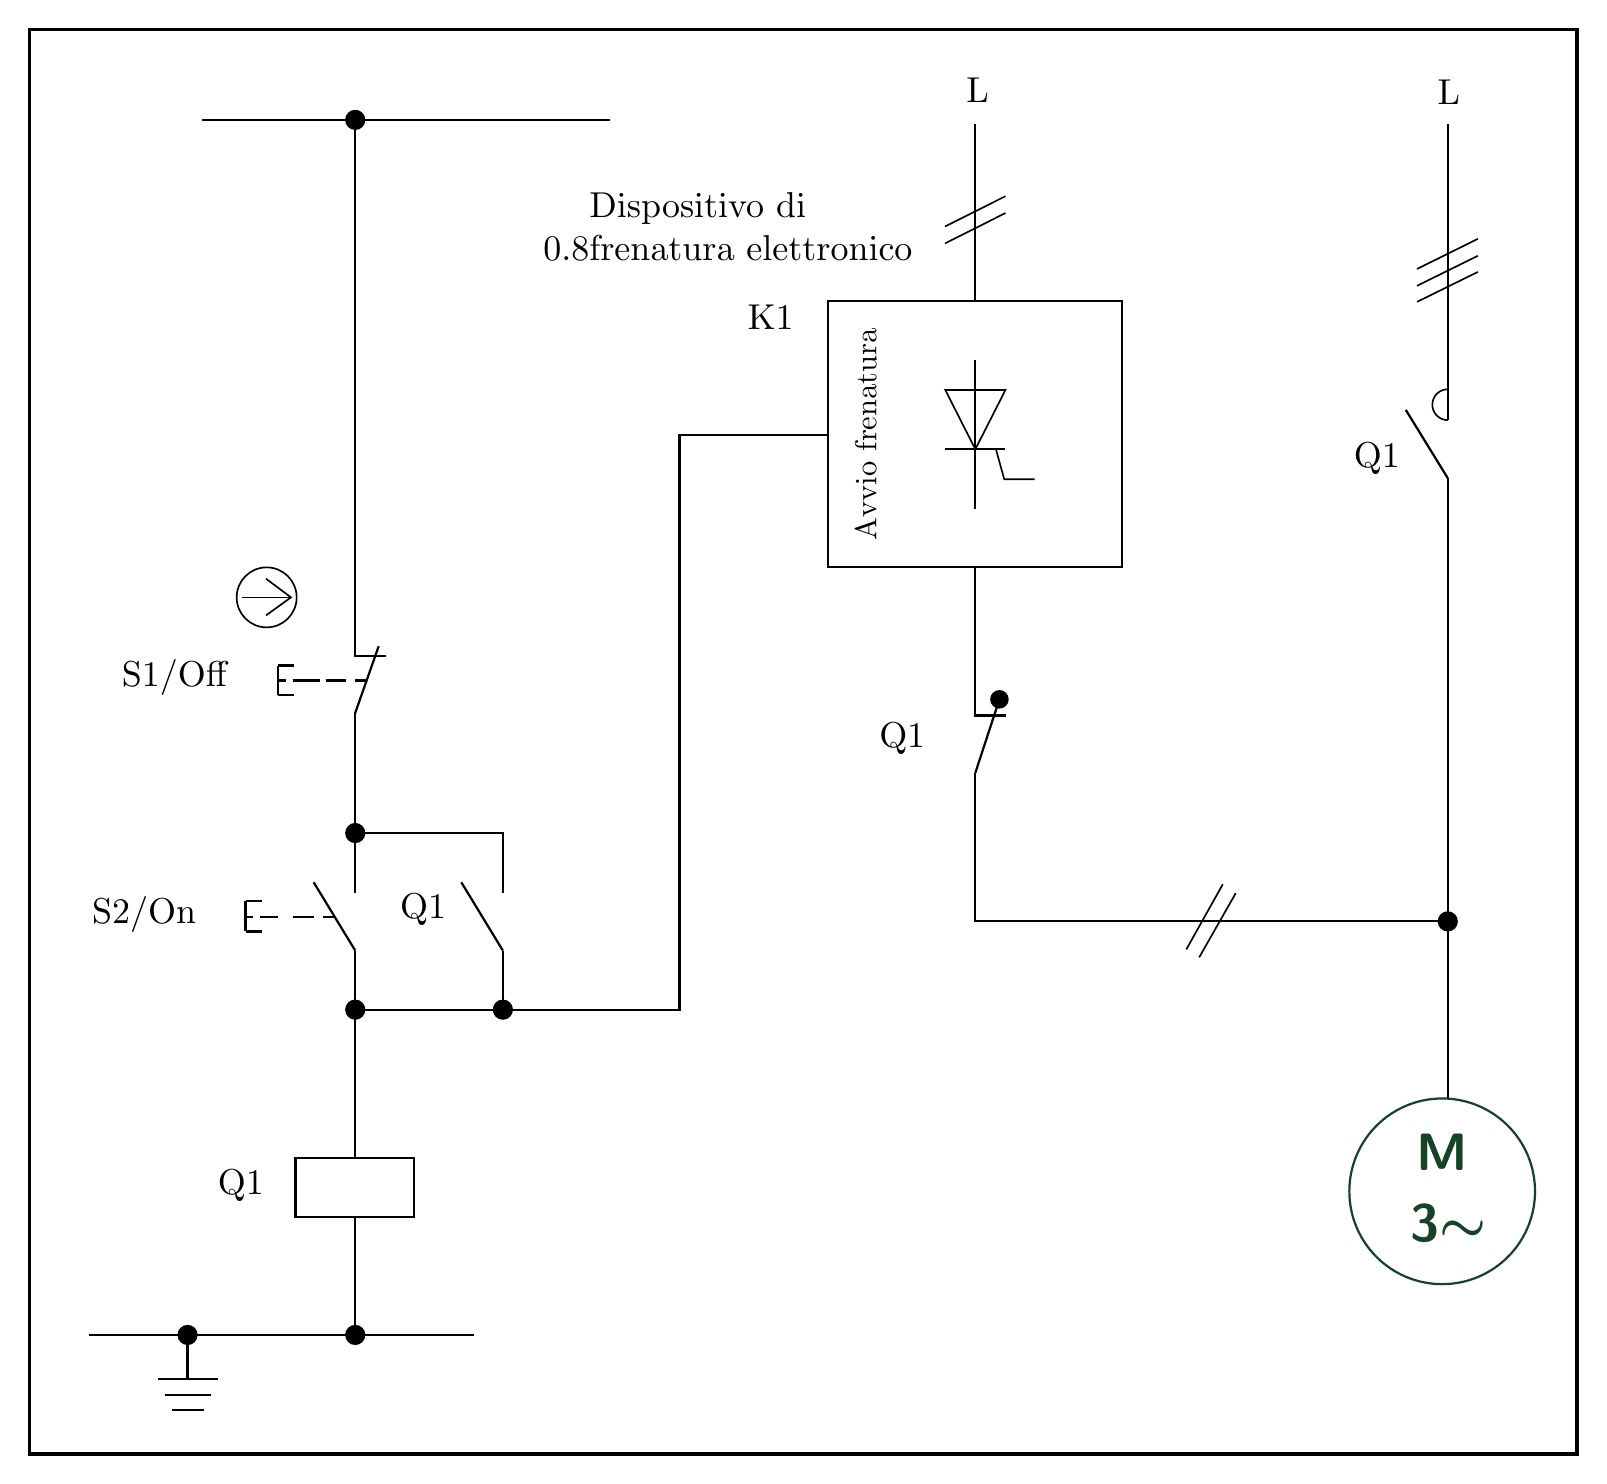
\begin{tikzpicture}[
  font=\normalsize,
  filo/.style={draw=black, line width=0.8pt},
  sottile/.style={draw=black, line width=0.6pt},
  etichetta/.style={inner sep=1pt, scale=1.3},
  testo/.style={align=left, inner sep=1pt, scale=1.3,
                execute at begin node=\setstretch{0.8}},
  nodo/.style={circle, fill=black, inner sep=0pt, minimum size=7.3pt}
]

%--------------------------------------------------------------
% Cornice
%--------------------------------------------------------------
\draw[draw=black, line width=1.2pt] (0.000,-0.000) rectangle (19.657,-18.093);

%--------------------------------------------------------------
% Circuito di comando: linea di alimentazione superiore
%--------------------------------------------------------------
\draw[filo] (2.193,-1.150) -- (7.371,-1.150);
\node[nodo] at (4.139,-1.150) {};

% S1/Off: pulsante di arresto (contatto di apertura) con simbolo
% di azionamento
\draw[filo] (4.139,-1.150) -- (4.139,-7.957) -- (4.529,-7.957);
\draw[filo] (4.137,-8.686) -- (4.437,-7.834);
\draw[filo] (4.139,-8.686) -- (4.139,-10.207);
\draw[filo] (3.157,-8.080) -- (3.157,-8.457);
\draw[filo] (3.157,-8.080) -- (3.357,-8.080);
\draw[filo] (3.157,-8.457) -- (3.357,-8.457);
\draw[filo] (3.157,-8.271) -- (3.257,-8.271);
\draw[filo] (3.343,-8.271) -- (3.691,-8.271);
\draw[filo] (3.763,-8.271) -- (4.023,-8.271);
\draw[filo] (4.137,-8.271) -- (4.283,-8.271);
\draw[sottile] (3.014,-7.214) circle (0.381);
\draw[sottile] (2.700,-7.214) -- (3.323,-7.214);
\draw[sottile] (3.006,-6.977) -- (3.323,-7.214) -- (3.006,-7.443);
\node[etichetta] at (1.843,-8.229) {S1/Off};

% S2/On (contatto di chiusura) e contatto di autoritenuta Q1
\node[nodo] at (4.139,-10.207) {};
\draw[filo] (4.139,-10.207) -- (4.139,-10.968);
\draw[filo] (3.611,-10.832) -- (4.139,-11.700);
\draw[filo] (4.139,-11.700) -- (4.139,-14.333);
\draw[filo] (2.746,-11.075) -- (2.746,-11.457);
\draw[filo] (2.746,-11.075) -- (2.954,-11.075);
\draw[filo] (2.746,-11.457) -- (2.954,-11.457);
\draw[filo] (2.746,-11.271) -- (2.843,-11.271);
\draw[filo] (2.932,-11.271) -- (3.157,-11.271);
\draw[filo] (3.354,-11.271) -- (3.621,-11.271);
\draw[filo] (3.729,-11.271) -- (3.879,-11.271);
\node[etichetta] at (1.457,-11.243) {S2/On};

\draw[filo] (4.139,-10.207) -- (6.014,-10.207) -- (6.014,-10.968);
\draw[filo] (5.486,-10.832) -- (6.014,-11.700);
\draw[filo] (6.014,-11.700) -- (6.014,-12.450);
\node[etichetta] at (5.000,-11.186) {Q1};

\node[nodo] at (4.139,-12.450) {};
\node[nodo] at (6.014,-12.450) {};
\draw[filo] (4.139,-12.450) -- (8.257,-12.450) -- (8.257,-5.153) -- (10.143,-5.153);

% bobina di Q1
\draw[filo] (3.381,-14.333) rectangle (4.886,-15.081);
\draw[filo] (4.139,-15.081) -- (4.139,-16.581);
\node[etichetta] at (2.686,-14.686) {Q1};

% linea di alimentazione inferiore e messa a terra
\draw[filo] (0.753,-16.581) -- (5.647,-16.581);
\node[nodo] at (4.139,-16.581) {};
\node[nodo] at (2.010,-16.581) {};
\draw[filo] (2.010,-16.581) -- (2.010,-17.139);
\draw[filo] (1.633,-17.139) -- (2.396,-17.139);
\draw[filo] (1.719,-17.343) -- (2.310,-17.343);
\draw[filo] (1.810,-17.539) -- (2.214,-17.539);

%--------------------------------------------------------------
% K1: dispositivo di frenatura elettronico
%--------------------------------------------------------------
\draw[filo] (12.014,-1.200) -- (12.014,-3.453);
\draw[sottile] (11.629,-2.504) -- (12.397,-2.119);
\draw[sottile] (11.629,-2.719) -- (12.397,-2.333);
\node[etichetta] at (12.043,-0.771) {L};
\node[testo, anchor=east] at (11.271,-2.507) {Dispositivo di\\ frenatura elettronico};

\draw[filo] (10.143,-3.453) rectangle (13.881,-6.833);
\node[etichetta] at (9.414,-3.657) {K1};
\node[inner sep=1pt, scale=1.1, rotate=90] at (10.624,-5.143) {Avvio frenatura};
% tiristore
\draw[sottile] (12.014,-4.200) -- (12.014,-6.090);
\draw[sottile] (11.633,-4.581) -- (12.396,-4.581) -- (12.014,-5.333) -- cycle;
\draw[sottile] (11.633,-5.333) -- (12.396,-5.333);
\draw[sottile] (12.276,-5.333) -- (12.381,-5.714) -- (12.767,-5.714);

% contatto di apertura di Q1
\draw[filo] (12.014,-6.833) -- (12.014,-8.714) -- (12.400,-8.714);
\draw[filo] (12.320,-8.509) -- (12.014,-9.443);
\node[nodo, minimum size=6.7pt] at (12.320,-8.509) {};
\draw[filo] (12.014,-9.443) -- (12.014,-11.329) -- (18.014,-11.329);
\draw[sottile] (14.693,-11.686) -- (15.157,-10.857);
\draw[sottile] (14.857,-11.786) -- (15.321,-10.971);
\node[etichetta] at (11.086,-9.014) {Q1};

%--------------------------------------------------------------
% Circuito di potenza: linea trifase L, contatto principale di Q1
% e motore M
%--------------------------------------------------------------
\draw[filo] (18.014,-1.200) -- (18.014,-4.961);
\draw[sottile] (17.624,-3.043) -- (18.396,-2.661);
\draw[sottile] (17.624,-3.257) -- (18.396,-2.876);
\draw[sottile] (17.624,-3.461) -- (18.396,-3.081);
\node[etichetta] at (18.029,-0.800) {L};
% contatto principale con apertura automatica
\draw[sottile] (18.014,-4.571) arc[start angle=90, end angle=270, radius=0.196];
\draw[filo] (17.481,-4.833) -- (18.014,-5.700);
\draw[filo] (18.014,-5.700) -- (18.014,-13.579);
\node[nodo] at (18.014,-11.329) {};
\node[etichetta] at (17.114,-5.457) {Q1};
% motore trifase
\draw[draw=verdemotore, line width=0.8pt] (17.943,-14.757) circle (1.179);
\node[inner sep=1pt, scale=1.9, text=verdemotore, font=\sffamily\bfseries\boldmath]
  at (17.943,-14.257) {M};
\node[inner sep=1pt, scale=1.9, text=verdemotore, font=\sffamily\bfseries\boldmath]
  at (18.029,-15.164) {3$\sim$};

\end{tikzpicture}
